
\documentclass[]{article}
\voffset=-1.2cm
\oddsidemargin=0.0cm
\textwidth = 490pt
\usepackage[utf8]{inputenc}
\usepackage[english]{babel}
\usepackage{framed}
\usepackage{graphicx}
\usepackage{enumerate}% http://ctan.org/pkg/enumerate
\usepackage{multicol}
\usepackage{amsmath}
\usepackage{amssymb}
%=========================================================================================== %

\begin{document}


\section*{MA4702 - Fundamentals of Mathematics and Limits}
%=============================== %

\noindent \textbf{Notation:}
\begin{framed}
	\begin{multicols}{2}
		\begin{itemize}
			\item $\mathbb{R}$ - All real numbers positive and negative
			\item $\mathbb{R}^+$ - All positive real numbers including $0$
			\item $\mathbb{R}^-$ - All negative real numbers including $0$
			\item $[a,b]$ - All real numbers $x$ such that $a \le x \le b$
			\item $(a,b)$ - All real numbers $x$ such that $a < x < b$
			\item $[a,\infty)$ - All real numbers $x$ such that $a \le x$
			\item $(a,\infty)$ - All real numbers $x$ such that $a < x$
		\end{itemize} 
	\end{multicols}
\end{framed}


\subsection*{Question 1 : Evaluation of Functions}
	
	\begin{itemize}
		\item[(i)] Evaluate the following function for x = -1,0,1 and 2 respectively.
		{
			\Large
			\[ f(x) = \frac{e^x - {e^{-x}}}{2} \]
		}
		\item[(ii)] Evaluate the function for each of the following values : $0.5,\;1,\;1.25,\;2$.
		{
			\Large
			\[f(x) =  \sqrt{1+e^{x}}  \]
		}
	\end{itemize}
	\subsection*{Question 2 : Floor and Ceiling Functions (Part A)}
\begin{framed}	\begin{itemize}
		\item $\lceil x\rceil$ : Ceiling function
		\item $\lfloor x\rfloor$  : Floor Function
		\item $\{x\}$ : Fractional Part of a number
		($\{x\} = x- \lfloor x\rfloor$)
	\end{itemize}
\end{framed}	\bigskip
	Complete the following table.
	\begin{center}
		{ \large 
			\begin{tabular}{|c|c|c|c|} \hline
				Value x & Floor $\lfloor x\rfloor$ & Ceiling  $\lceil x\rceil$ & Fractional $ \{ x \} $\\ \hline
				-1.4  &	-2	&-1&	 \\ \hline
				2.3&	&		& \\ \hline
				7/9&		&		& \\ \hline 
				-16/3&		&		& \\ \hline
				0 & 	&		& 0 \\ \hline
				1 & 	&	1	& \\
				\hline
			\end{tabular} 
		}
	\end{center}
	\bigskip
	\subsection*{Question 3 : Floor and Ceiling Functions (Part B)}
	Provide some values for $x$ and $y$ that \textbf{contradict} the following statement.
	\[ \lfloor x + y \rfloor  = \lfloor x\rfloor + \lfloor y \rfloor\]
	
	\noindent If the values of x and y were integers, would the equation be true for all values of $x$ and $y$?
	
	%------------------------------- % 



	\subsection*{Question 4 : Laws for Logarithms}
	The following laws are very useful for working with logarithms.\bigskip
	\begin{framed}
	\begin{multicols}{2}
	\begin{enumerate}
		\item $\mbox{log}_b(X)$ + $\mbox{log}_b(Y)$ = $\mbox{log}_b(XY)$\bigskip
		\item $\mbox{log}_b(X)$ - $\mbox{log}_b(Y)$ = $\mbox{log}_b(X / Y)$ \bigskip
		\item $\mbox{log}_b(X^Y)$ = $Y \mbox{log}_b(X)$
		
		\item $\mbox{log}_b(X) = 1 $ when $b=X$
	\end{enumerate}
	\end{multicols}
	\end{framed}

\bigskip
\large
\noindent Use the Laws of Logarithms to evaluate the following expressions:

	\begin{multicols}{2}
		\begin{itemize}
		\item[(i)] $\mbox{log}_2(8)$
		\item[(ii)] $\mbox{log}_2(\sqrt{128})$
		\item[(iii)] $\mbox{log}_2(64)$
		\item[(iv)] $\mbox{log}_5(125)$ +   $\mbox{log}_3(729)$
		\item[(v)] $\mbox{log}_2(64/4)$
		\item[(vi)] $\mbox{log}_3(\frac{1}{81})$
				\end{itemize}
		\end{multicols}
%------------------------------- %
	\subsection*{Question 5 : Cross Multiplication}
	Solve the following equations for A and B where $A,B \in \mathbb{R}$
	\begin{multicols}{2}
	\[ \mbox{(i)     } \frac{11}{x^2 - 4x - 12} = \frac{A}{x-6} + \frac{B}{x+2}\]
	
	\[ \mbox{(ii)    }\frac{2x + 5}{x^2 - 4x - 12} = \frac{A}{x-6} + \frac{B}{x+2}\]
	
	\[ \mbox{(iii)     }  \frac{1}{(n)(n+1)} = \frac{A}{n} + \frac{B}{n+1}\]
	
	\[ \mbox{(iv)    }\frac{2}{(n+1)(n+3)} = \frac{A}{n+1} + \frac{B}{n+3}\]
	\end{multicols}
%---------------------------------------------------------- %
\subsection*{Question 6 : Exponential and Logarithm Exercises}

\begin{multicols}{2}
\begin{itemize}
	\item[(i)] Find the value of $x$
	\[e^{2x-5} = 3. \]
		
	\item[(ii)] Find the value of $x$
	\[ln(e^x+2) = 4\]
	
	\item[(iii)] Find the value of $x$
	\[log_3(2x - 1) + log_3(5) = 3\]
	
	\item[(iv)] Find the value of $x$
	\[log_2(x + 1) + log_2(5) = 3\]
\end{itemize}
\end{multicols}
\subsection*{Question 7 : Review of Differentiation}
\begin{multicols}{2}
\begin{itemize}
\item[(i)] $f(x) = e^{4x}$
\item[(ii)] $f(x) = \cos(4x)$
\item[(iii)] $f(x) = \sin(3x)$
\item[(iv)] $f(x) = e^{4y} \cos(4x)$
\item[(v)] $f(y) = e^{4y} \cos(4x)$
\end{itemize}
\end{multicols}

\subsection*{Question 8 : Expressing Repeating Decimals as Fractions}
Express the following numbers as fractions. For example $ 0.77777... = \frac{7}{9}$

\begin{multicols}{2}
	\begin{itemize}
		\item[(i)] $0.29292929....$
		\item[(ii)] $0.475475475....$
		
		\item[(iii)] $0.4545454545.....$
		\item[(iv)] $0.473473473.........$
	\end{itemize} 
\end{multicols}

\newpage

	%------------------------------- %
\subsection*{Question 9 : Evaluate the following limits}

\begin{multicols}{2}
	\begin{itemize}
		\item[(i)] \[ \lim_{x\to 5} (x^2)\]
		
		% - 5^2=\mathbf{25}
		\item[(ii)] \[ \lim_{x\to 2} (4x^2 - 3x+1)\]
		% -4(4)-2(3)+1=16-6+1=\mathbf{11}
		
		
		\item[(iii)]\[\lim_{x \to 4 } x  + 5 \]
		% Answer 9 
		\item[(iv)]\[\lim_{x \to 2 } 2x  - 1 \]
		% Answer 1
		\item[(v)]\[\lim_{x \to 2 } \frac{x^2-4}{x-2}\]
		%Answer 4
		\item[(vi)]\[\lim_{x \to 3 } \frac{x^2-4x +3}{x-3}\]
		% Answer 2
		
		\item[(vii)]\[\lim_{x \to \infty } \frac{x+4}{x-4}\]
		% Answer 0
		\item[(viii)]\[\lim_{x \to \infty } \frac{x^3-4}{x-1}\]
		% Answer 0
		\item[(ix)] \[\lim_{x \to \infty } \frac{x^2-1}{x-1} \]
		% Answer 2 	
		
		\item[(x)] \[ \lim_{x \to \infty} \frac{2x^2 +8}{5x^2 - 7x} \] 
		
		\item[(xi)]\[ \lim_{x \to \infty} \frac{3x^2 +7x^3}{x^2 +5x^4} \] 
		
		\item[(xii)] \[ \lim_{x \to \infty} \frac{2x^2 - 8x }{4x^2 - 7} \]
		
		
		\item[(xiii)] \[ \lim_{x \to \infty} \frac{x-3}{x^2 - 9} \]
	\end{itemize}
\end{multicols}
% http://en.wikibooks.org/wiki/Calculus/Limits/Solutions#Basic_Limit_Exercises

%================================================================= %
\newpage

\subsection*{Question 10:  Sequences and Series}

\begin{enumerate}
	\item[(i)] Find the sum of the first 10 numbers of this arithmetic series: $1 + 11 + 21 + 31 + \ldots$
	
	\item[(ii)] 
	The second term $u_2$ of a geometric sequence is 21.
	
	The third term $u_3$ is -84.
	\begin{itemize}
		\item Find the common ratio 
		\item Find the first and fourth term
	\end{itemize}
	%- Page 16
	
	\item[(iii)] Three consecutive terms of an arithmetic series are \[4x - 1, 2x +11, 3x + 41. \]
	Find the value of x.
	%answer is 460
	
	\item[(iv)] Find the sum of the following geometric series: 
	\[3 + 6 + 12 + 24 + \ldots + 1536\]
	
	%----------------------------------%
	\item[(v)] 
	
	In an arithmetic sequence, three consecutive terms have a sum of - 9 and a product of 48.
	Find the common difference $d$ for these terms.
	\\
	\textit{\textit{Hint : Write terms as $x-d,x,x+d$}}
	%----------------------------------%
	\item[(vi)]
	The first three terms of an arithmetic sequence are 6,-9 and x.
	The first three terms of a geometric sequence are 6, x, y.
	Find the value of $x$ and the value of $y$.
	
	%---------------------------------%
	\item[(vii)]
	Find the sum to infinity of the geometric series
	
	\[ 1 + \bigg(\frac{2}{3}\bigg) + \bigg(\frac{2}{3}\bigg)^2 + \bigg(\frac{2}{3}\bigg)^2 + \ldots \]
	%-----------------------------------%
	\item[(viii)]
	The first three terms of a geometric series are
	
	\[ x-2 , 2x+3, 7x \]
	
	Find both of the possible values of $x$
	
	%- Page 27
	
	%----------------------------------%
	\item[(ix)]
	The $n-$th term of an arithmetic is $3n+2$
	
	Find $S_n$ the sum of the first $n$ terms, in terms of $n$
\end{enumerate}
\newpage


\subsection*{Question 11 : Convergence of a Sequence}

\begin{framed}
	A sequence $u_n$
	is said to converge to a limit $L$ where $L \neq \infty$ if
	\[ \lim_{n \to \infty } u_n = L \]
	
	
	
	
	If a sequence does not converge then it is said to be divergent. \end{framed}
%
%\begin{itemize}
%\item  Unless explicity told to use the Ratio test, you may use this approach.
%\end{itemize}
Test the following sequences for convergence. see page 14 of notes for more details.
\begin{multicols}{2}
	\begin{itemize}
		\item[(i)] \[u_n = \frac{2n-1}{4n+3}\]
		
		\item[(ii)] \[u_n = \frac{n+5}{3n+4}\]
		
		\item[(iii)] \[u_n = \frac{n+4}{2n^3 + n +3}\]
		
		\item[(iv)] \[u_n = \frac{n^2 +5n }{n^2 + 2n -1}\]
		
		\item[(v)] \[u_n = \frac{2n^3+1}{2n^3 +3n +4 } \]
		
		\item[(vi)]\[u_n =  \frac{2n^4+1}{n^3 +2n^2 -1 } \]
		
	\end{itemize}	
\end{multicols}
%====================================%


\subsection*{Question 12 : Partitioning of Summations}
\begin{framed}
	
	For some integers $m$ and $n$, with $m<n$.
	
	\[ \sum^{i=n}_{i=1} u_{i} = \sum^{i=m}_{i=1} u_{i} + \sum^{i=n}_{i=m+1} u_{i}\]
	
	Suppose $n=100$ and $m=50$
	
	\[ \sum^{i=100}_{i=1} u_{i} = \sum^{i=50}_{i=1} u_{i} + \sum^{i=100}_{i=51} u_{i}\]
	
\end{framed}
\newpage

\noindent Compute the following 

\begin{multicols}{2}
	\begin{itemize}
		
		
		\item[(i)]	\[ \sum_{i=1}^{30} i \]
		\item[(ii)]  
		
		\[ \sum_{i=1}^{65} i \]
		
		\item [(iii)] 
		
		\[ \sum_{i=1}^{37} i \]
		
		
		\item [(iv)] 
		
		\[ \sum_{i=38}^{65} i \]
		
	\end{itemize}
\end{multicols}




\subsection*{Question 13 : Sum to Infinity Exercises}
Compute the summations of the following infinite series
\begin{multicols}{2}
	\begin{itemize}
		\item[(i)] $1 + 0.2 + 0.04 + \ldots$
		\item[(ii)] $1 - 0.2 + 0.04 - \ldots$
		
		\item[(iii)] $20 + 5 + 1.25 + \ldots$
		\item[(iv)] $- 20 + 5 - 1.25 + \ldots$
	\end{itemize} 
\end{multicols}
\bigskip
\subsection*{Question 14 : Summation of an Infinite Series}

Find the value to which each of the following series converges.

\[\sum_{n=1}^{\infty} \frac{3}{4^{n-1}}\]
%- http://en.wikibooks.org/wiki/Calculus/Sequences_and_Series/Exercises

	\subsection*{Question 15 : The Ratio test}


	\begin{framed}
		\noindent For a series with general term $u_n$, if
		
		\[ \lim_{n \to \infty } \left| \frac{u_{n+1}}{u_n} \right| = r\]
		then
		
		\begin{itemize}
			\item the series converges (absolutely) if $r<1$
			\item the series diverges if $r>1$ (or if r is infinity)
			\item the series could do either if $r=1$, so the test is not conclusive.
		\end{itemize}
	\end{framed}
\noindent \textit{This formula will be given in the back of the exam paper. However the indications on how to interpret $r$ will not be given.}
	\begin{framed}
		\subsubsection*{Example}
		Suppose that the following term is the general term for a series. Test this series for convergence
		
		\[u_n=\frac{n!n!}{(2n)!}\]
		then
		
		\[\frac{u_{n+1}}{u_n}=\frac{(n+1)^2}{(2n+1)(2n+2)}=\frac{n+1}{4n+2} \]
		\[ \to \frac{1}{4}\]
		so this series converges.
	\end{framed}
	
	
	
	
	\noindent Use the Ratio Test to test the following series for convergence
	\begin{multicols}{2}
		\begin{itemize}
			\item[(i)] 
			\[\sum^{\infty}_{n=1} \frac{x^{n+1}}{4^n} \]
			\item[(i)] 
			\[\sum^{\infty}_{n=1} \frac{4^n}{(n+1)!} \]
			
			\item[(iii)] \[\sum^{\infty}_{n=1} \frac{5^n }{n!} \]
			
			
			\item[(iv)] \[\sum^{\infty}_{n=1} \frac{n+1}{2^n} \]
			
		\end{itemize}
	\end{multicols}
	
	\begin{itemize}
		\item[(v)] Use the Ratio test to find the values for $x$ for which the series  is convergent
		\[\sum^{\infty}_{n=1} \frac{x^{n} }{n+2} \]
		
	\end{itemize}
	

\newpage



\subsection*{Question 16 : Evaluation of telescoping series}

Find the sum of the following telescoping series
\begin{multicols}{2}
	\begin{itemize}
		\item[(i)]
		\[  \sum^{\infty}_{n=1}   \frac{3}{(3n+1)(3n+4)}  \]
		
		\item[(ii)]
		\[  \sum^{\infty}_{n=1}   \frac{4}{(2n+1)(2n+3)}  \]
		
		\item[(iii)]
		\[  \sum^{\infty}_{n=1}   \frac{5}{(5n+1)(5n+6)}  \]
		
		\item[(iv)]
		\[  \sum^{\infty}_{n=1}  \frac{6}{(6n+1)(6n+7)}  \]
		.
	\end{itemize}
\end{multicols}

%=========================================================== %
\bigskip
\subsection*{Question 17 : Evaluation of Telescoping Series}
Answer the following questions
\begin{itemize}
	% % Revise Cross Multiplication
	\item[(i)] Show that, where $r \neq \pm 1$.
	\[ \frac{2}{r^2-1} =  \frac{1}{r-1} - \frac{1}{r+1} \]
	% \item[(ii)] Hence, find the following summation
	
	% \[  \sum^{n}_{r=2} \frac{2}{r^2+1} \]
	\item[(ii)] Hence, evaluate the following summation
	\[  \sum^{n}_{r=2} \frac{2}{r^2-1} \]
	\item[(iii)] Hence, evaluate the following summation
	\[  \sum^{\infty}_{r=2} \frac{2}{r^2-1} \]
\end{itemize}

\subsection*{Question 18 : Evaluation of terms in a Maclaurin Series}
\large
\begin{itemize}
	\item[(i)] Evaluate the following Macluarin Series for $n=\{1,2,3\}$.
\end{itemize}
\begin{figure}[h!]
	\centering
	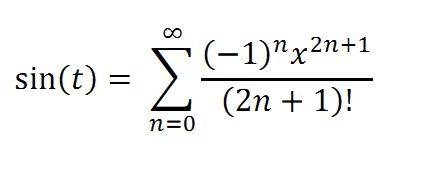
\includegraphics[width=0.30\linewidth]{macl3}
	%	\caption{}
	\label{fig:macl3}
\end{figure}

%========================================================================= %
\newpage

%==========================================================================%
%
%
%
%\section*{MA4702 - Part 4 - Function}
%
%\begin{itemize}
%\item	Functions
%\item	Domain and Range
%\item	Odd and Even Functions
%\item 	Composite Functions 
%\item	Inverse Functions
%\item 	Hyperbolic Functions
%\item	Osborne Rules
%	
%\end{itemize}
\subsection*{Question 19 : Functions}

\subsubsection*{Part A - Functions}
Consider the function f(x) where \[ f(x) = \frac{1}{\sqrt{3x-6}} \]




\begin{itemize}
	\item[(i)] Find the domain and range of f(x)
	\item[(ii)] Find $f(3x^2 + 2)$ and simplify
\end{itemize}
%================================================================================%


\subsubsection*{Part B - Functions}
Consider the functions $f(x) = \sqrt{2x-6}$ and  $g(x) = log_e(2x + 1)$

\begin{itemize}
	\item[(i)]Find $f(4 – 2x^2)$ and simplify answer.
		\item[(ii)] Write down the domain and range of f(x).
		\item[(iii)] Determine $g^{-1}(x)$, the inverse of g(x).
\end{itemize}

%================================================================================%


\subsubsection*{Part C - Composite Functions}
Consider the functions $f(x) = \sqrt{2x-8}$, and $g(x) = 2x^2 + 4$.
\begin{itemize}
	\item[(i)] Find the composite function $f \circ g(x)$ and $g \circ f(x)$,  simplifying your answer as much as possible.
	\item[(ii)] Determine $f^{-1}(x)$, the inverse of f(x).
\end{itemize}

%================================================================================%











% (iii) Find g -1(x) the inverse of g(x). 10




%-----------------------------------------------------------------
%================================================================== %
\subsection*{Question 20 : Functions}
\begin{itemize}
\item[(i)] Find $f^{-1}(x)$  the inverse of the function

\[f(x) = \frac{1}{2x-5}\]

\item[(ii)] Find the domain and the range of the function:

\[f(x) =  7 + 2 sin(x)\]

\item[(iii)] Find $f^{-1}(x)$  the inverse of the function

\[f(x) = \sqrt{2x + 3} \]

\item[(iv)] Find $f^{-1}(x)$ the inverse of the function

\[f(x) = e^{3x}\]

\item[(v)] Find the domain and the range of the function:

\[ f(x) = 1-x^2 \]

\item[(vi)] Find the domain and the range of the function:

\[f(x) = ln(x)\]

\end{itemize}

%================================================================ %
	\subsection*{Question 21 : Hyperbolic Functions - Proof of Identities}
	Recall 
	\begin{framed}
		\begin{multicols}{2}
			\[ (a-b)^2 = a^2 -2ab +b^2 \]
			
			\[ (a+b)^2 = a^2 + 2ab +b^2 \]
			
			\[ (e^x)^2  = e^{2x} \]
			
			\[  (e^x) \times (e^{-x}) = e^{x-x} =e^0  =1  \]
		\end{multicols}
	\end{framed}
\noindent	Using their definition in terms of exponentials, prove the following 
	hyperbolic identity:
	\begin{itemize}
			\item[(i)] Show that \[\sinh2x = 2\sinh(x) \cosh(x) \]
		\item[(ii)] Show that \[ \sinh^2(x) = \frac{1}{2} \big[ \cosh(2x)-1 \big]\]
			\item[(iii)] Show that \[ \cosh^2(x) - \sinh^2(x) = 1\]
	%	\item[(iv)] Show that \[ \cosh^2 x = \cosh2x + \sinh2x\]	
		\item[(iv)] Show that \[ \cosh(x+y) = \cosh(x)\cosh(y) + sinh(x)sinh(y)\]
	
		% %- http://www.sosmath.com/trig/hyper/hyper01/hyper01.html
		
	\end{itemize}
\newpage



	

	\subsection*{Question 22 : Inverse of Functions}
	
	\begin{framed}
		\textbf{Procedure}
		\begin{itemize}
			\item	To determine $f^{-1}(x)$ when given a function $f$, substitute $f^{-1}(x)$ for x and substitute x for f(x).
			\item Then solve for $f^{-1}(x)$, provided that it is also a function.
		\end{itemize}
	\end{framed}
	
	%=======================================%
	\begin{framed}
		
		\noindent	\textbf{Example:}\\ Given $f(x) = 2x - 7$, find $f^{-1}(x)$.
		\\
		\noindent Substitute $f^{-1}(x)$ for x and substitute x for f(x). Then solve for $f^{-1}(x)$:
		
		\[f(x) = 2x - 7\,\]
		\[x  = 2[f^{-1}(x)] - 7\,\]
		\[x + 7  = 2[f^{-1}(x)]\,\]
		\[\frac{x + 7}{2} = f^{-1}(x)\,\]
	\end{framed}
	\begin{itemize}
		\item[(i)] Find $f^{-1}(x)$ the inverse of the function 
		\[f(x) = \frac{1}{2x-5}\]
		\item[(ii)]  given that $g(x) = log_e (4x)$ , find $g^{-1} (x)$ the inverse function of g(x).
	\end{itemize}
	
	%=================================================================================== %
	
	
	
\subsection*{Question 23 : Even and Odd Functions}
Check whether the following functions are even, odd or neither.
\begin{multicols}{3}
	\begin{itemize}
		\item[(i)] \[f(x) = \frac{4}{x^2+1}\]
		\item[(ii)] \[f(x) = sin(4x) \]
		\item[(iii)] \[f(x) = -cos(3x) \]
		\item[(iv)] \[f(x) = \frac{3x+2}{4x+3} \]
		\item[(v)] \[f(x) =  \frac{e^{x} - e^{-x}}{2}\]
		\item[(vi)] \[f(x) = \frac{x}{x^2-4} \]
	\end{itemize}
\end{multicols}

\subsection*{Question 24 : Calculations for the Ratio Test}

For each of the following terms, given as $u_n$, state $u_{n+1}$ and hence calculate a simplified expression for $r$, where 
{
	\Large
\[ r = \frac{u_{n+1}}{u_n}\]
}
{
	\Large
\begin{multicols}{2}
\begin{itemize}

	
	
	\item[(i)]	$u_n= 2^n$\smallskip
	
		\item[(ii)] $u_n=n!$\smallskip
	
	\item[(iii)] $u_n = \displaystyle{\frac{(n+1)!}{2^n}} $\smallskip
	
		\item[(iv)] $u_n = n! \times n! $
	
\item[(v)]	$u_n = \displaystyle{\frac{4^n}{2^n}} $
	
	
	\item[(vi)]$u_n = \displaystyle{\frac{4^n}{(2n)!}} $
	
	
	\item[(vii)]$u_n = \displaystyle{\frac{5^n}{n!} }$ (2010 Exam)
	
	
	\item[(viii)]$u_n = \displaystyle{\frac{x^n}{n+1} }$ (2005 Exam)
	
	\item[(ix)]$u_n =\displaystyle{ \frac{n+1}{2^n}} $ (2009 Exam)
	
	\item[(x)]$u_n = \displaystyle{\frac{4^n}{(n+1)!}} $ (2007 Exam)
\end{itemize}
\end{multicols}
\smallskip
}
%	\item[(i)]  $u_n = \displaystyle{n^2}$\smallskip
%	\item[(ii)] $u_n = \displaystyle{2^n}$ \smallskip
%	\item[(iii)] $u_n = \displaystyle{\frac{2^n}{n^2}}$ \smallskip
%	\item[(iv)] $u_n = (2n)!$
%	\item[(v)] $u_n = \displaystyle{\frac{2^n}{n!}}$ \smallskip
%	\item[(vi)] $u_n = \displaystyle{\frac{2^n \times n}{n!}}$\smallskip
%	\item[(vii)] $un = n! \times n!$
%	\item[(viii)] $u_n = \displaystyle{\frac{2^{n+1} \times n^2}{ 4^n \times n!}}$

%================================================================== %

\subsection*{Question 25 : Functions - Part A}
%\begin{framed}
%	\begin{enumerate}
%		\item Trigonometric Functions and the Unit Circle
%		\item Domain, Codomain and Range
%		\item One to One and Onto Functions (using Arrow Diagrams)
%		\item Special Functions
%		\item Inverting a Function
%	\end{enumerate}	
%\end{framed}
%===================================================%

\begin{figure}[h!]
	\centering
	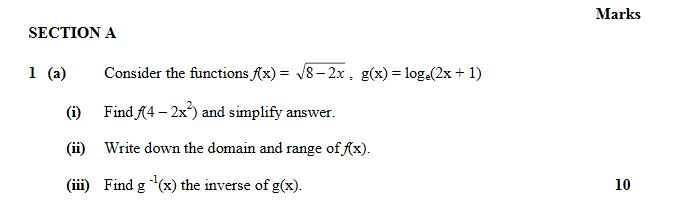
\includegraphics[width=1\linewidth]{Week7tut1}
\end{figure}
\newpage
\subsection*{Question 25 : Functions - Part B}
\begin{figure}[h!]
	\centering
	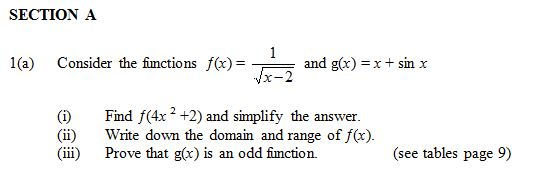
\includegraphics[width=1\linewidth]{Week7tut2}
\end{figure}

%\subsection*{Question 25 : Functions - Part C}
%\begin{figure}[h!]
%	\centering
%	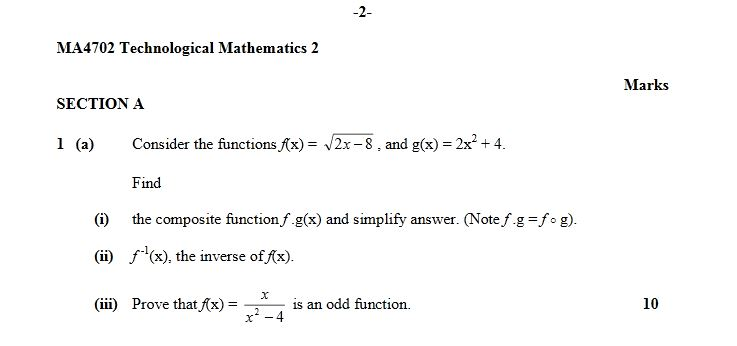
\includegraphics[width=1\linewidth]{Week7tut3}
%\end{figure}

\newpage
%==============================================================================%



%=========================== %
		\subsection*{Question 26 : Domain and Ranges of Functions}
% - https://en.wikibooks.org/wiki/Algebra/Functions#Domain_and_Range
% - http://www.regentsprep.org/regents/math/algtrig/ATP7/fogprac.htm
			Find the domain and the range of the functions:
			\begin{multicols}{2}
	\begin{enumerate}[(i)]
%number 1
\item $f( x )= x - 2$ \,\, $g( x )= -2 x$

%number 2
\item $f( x )= x^2 - 4$\,\, $g( x )= - x^2 - 4$

%\item $f( x )= x^2 - 2$, $g( x)= -0.5 x^2 - 2 x$

%\item $f( x )= x^3$ , $g( x )= - x^3 - 4 x^2 - 4 x$

\item $f( x )= \sqrt{x}$ \,\, $g( x )= \sqrt{x - 2}$

%\item $f( x )= \sqrt{x +2}$ , $g( x )=  \sqrt{x - 2}-1$


%number 4
\item $f( x ) =  \sin x$ \,\, $g( x ) =  -2 \sin x$

%number 5
\item $f( x ) =  \cos x$ \,\, $g( x ) =  \cos^2(x)$

%number 6
\item $f( x ) =  e^{x}$\,\, $g( x) =  e^{x}- 2$


%\item $f( x ) =  e^{-x}$, $g( x) =  e^{-x}- 2$
%
%
%\item $f( x ) =  2 e^x$, $g( x ) = \frac{1}{e^x - 1}$
%
%
%\item $f( x ) = | x |$, $g( x) =  | x - 2|$
%
%\item $f( x ) = | x |- 2$, $g( x) =  | x - 3 |- 1$

\end{enumerate}
\end{multicols}		\smallskip
		\subsection*{Question 27 : Domain and Ranges of Functions}
			Find the domain and the range of the functions:
\begin{multicols}{2}
		\begin{enumerate}[(i)]
		\item $f(x) = 8 - 2 \sin(x)$ 	

		\item $f(x) = 5 - 2 \cos(2x)$ 
			\item $f(x) =  2 \cos(x)- 6$ 

		\item $f(x) = 7 + 2 \sin(3x)$ 
		
		\item $f(x) = 5\sin(x) - 2 \cos(x)$ 
				
		\item $f(x) = \cos^2(x) +  \sin^2(x)$ 
				\item $f(x) = \cos^2(x) -  \sin^2(x)$ 
	\end{enumerate}	
\end{multicols}		
		\smallskip
	\subsection*{Question 28 : Evaluation of trigonometric values}
	Evaluate the following values. \textit{you may use your calculator.}
	\begin{multicols}{2}
		\begin{itemize}
			\item[(i)] $\cos (\pi/2)$
			\item[(ii)] $\sin (3\pi/4)$
			
			\item[(i)] $\tan (\pi/6)$
			\item[(ii)] $\cos (1.5 \pi)$
		\end{itemize} 
	\end{multicols}
	\bigskip	


\newpage
\subsection*{Question 29 : Composite Functions}
Determine the values of $f \circ g(2)$ and $g \circ f(x)$. Henxe or otherwise, evaluate $f \circ g(2)$ and $g \circ f(2)$.
\begin{multicols}{2}
	\begin{enumerate}[(i)]
	\item $f(x) = X^2 + 1$ and $g(x)= 2x$
		\item $f(x) = \sqrt{x+1}$ and $g(x)=x^2$
		\item $f(x) = x^2-1$ and $g(x) = 2x+1$
		
				\item $f(x) = 5x $ and $g(x)=x^2+1$
	\item $f(x) = -4x+9$ and $g(x) = 2x-7$
				%	\item $f(x) = -4x+9$ and $g(x) = 2x-7$
						\item $f(x) = e^x$ and $g(x)=\ln(x)$
						\item  $f(x) = x^2+1$ and $g(x) = 1-3x$
						\item $f(x) = \sin(\pi x)$ and $g(x) = 2x+1$
	\end{enumerate}	
\end{multicols}	
\medskip

\subsection*{Question 30 : Inverse Functions}

\begin{multicols}{2}
	\begin{enumerate}[(i)]
\item	$f(x) = 2x$
\item	$f(x) =e^x$
\item	$f(x) = x-3$
	
\item	$f(x) =\cos(x)$
\item	$f(x) = \sin^{-1}(x)$
\item  ${f(x) = \displaystyle \frac{1}{x-1}}$
	
\item	$f(x) = x^2+2$
\item	$f(x) = \sin^{-1}(2x)$
\item	$f(x) = 3 e^{2x}$
\item $f(x) = \sqrt{2x+3}$
\item $f(x) = \log_e{4x}$
\item $ \displaystyle f(x) = \frac{-2}{x-5}$
	\end{enumerate}	
	\smallskip
\end{multicols}
\noindent \textbf{Selected Solution}
	\begin{enumerate}[(i)]
		\item For the function $f(x) = 2x$ the inverse function is $f^{-1}(x) = x/2$.
		\item For the function	$f(x) =e^x$ the inverse function is  $f^{-1}(x) = \log_e(x) = \ln(x)$.
		\item For the function	$f(x) = x-3$ the inverse function is $f^{-1}(x) = x+3$
		
		\item For the function	$f(x) =\cos(x)$ the inverse function is $f^{-1}(x) = \cos^{-1}(x)$.
		\item For the function	$f(x) = \sin^{-1}(x)$ the inverse function is $f^{-1}(x) = \sin(x)$.
		
	
\end{enumerate}
\newpage
\subsection*{Question 31 : Revision of Product, Quotient and Chain Rule}
\begin{multicols}{2}
	\begin{enumerate}[(i)]
			%%%===Product Rule===		
	\item		 \[ f(x) = (x^4+4x+2)(2x+3) \,\] %%%={{noprint|ˆt10x^4+12x^3+16x+16</math>}}}}
	\item		 \[ f(x) = (2x-1)(3x^2+2) \,\] %%%={{noprint|ˆt18x^2-6x+4</math>}}}}
	\item		 \[ f(x) = (x^3-12x)(3x^2+2x) \,\] %%%={{noprint|ˆt15x^4+8x^3-108x^2-48x</math>}}}}
	\item		 \[ f(x) = (2x^5-x)(3x+1) \,\] %%%={{noprint|ˆt36x^5+10x^4-6x-1</math>}}}}
%	\item		. \[ f(x) = (5x^2+3)(2x+7)\,\] %%%={{noprint|ˆt30x^2+70x+6</math>}}}}
%	\item		. \[ f(x) = 3x^2(5x^2+1)^4 \,\] %%%={{noprint|ˆt6x(25x^2+1)(5x^2+1)^3</math>}}}}
%	\item		. \[ f(x) = x^3(2x^2-x+4)^4 \,\] %%%={{noprint|ˆtx^2(2x^2-x+4)^3(22x^2-7x+12)</math>}}}}
%	\item		. \[ f(x) = 5x^2(x^3-x+1)^3 \,\] %%%={{noprint|ˆt5x(x^3-x+1)^2(11x^3-2x+1)</math>}}}}
%	\item		. \[ f(x) = (2-x)^6(5+2x)^4 \,\] %%%={{noprint|ˆt2(x-2)^5(2x+5)^3(10x+7)</math>}}}}
	\item		\[ f(x) = \frac{2x+1}{x+5} \,\] %%%={{noprint|ˆtf'(x)=\frac{9}{(x+5)^2}</math>}}}}
	\item		 \[ f(x) = \frac{3x^4+2x +2}{3x^2+1} \,\] %%%={{noprint|ˆtf'(x)=\frac{18x^5+12x^3-6x^2-12x+2}{(3x^2+1)^2}</math>}}}}
	\item		 \[ f(x) = \frac{x^\frac{3}{2}+1}{x+2} \,\] %%%={{noprint|ˆtf'(x)=\frac{x\sqrt{x}+6\sqrt{x}-2}{2(x+2)^2}</math>}}}}
	%% \item		ˆtd(u) = \frac{u^3+2}{u^3} \,\] %%%={{noprint|ˆtd'(u)=-\frac{6}{u^4}</math>}}}}
	\item		\[ f(x) = \frac{x^2+x}{2x-1} \,\] %%%={{noprint|ˆtf'(x)=\frac{2x^2-2x-1}{(2x-1)^2}</math>}}}}
	\item		 \[ f(x) = \frac{x+1}{2x^2+2x+3} \,\] %%%={{noprint|ˆtf'(x)=\frac{-2x^2-4x+1}{(2x^2+2x+3)^2}</math>}}}}
	\item		 \[ f(x) = \frac{16x^4+2x^2}{x} \,\] %%%={{noprint|ˆtf'(x)=48x^2+2</math>}}}}
	\item		\[ f(x) = (x+5)^2 \,\] %%%={{noprint|ˆtf'(x)=2(x+5)</math>}}}}
	%% 32. ˆtg(x) = (x^3 - 2x + 5)^2 \,\] %%%={{noprint|ˆtg'(x)=2(x^{3}-2x+5)(3x^{2}-2)</math>}}}}		
	\item 		 \[ f(x) = \sqrt{1-x^2} \,\] %%%={{noprint|ˆtf'(x)=-\frac{x}{\sqrt{1-x^{2}}}</math>}}}}
	\item 		 \[ f(x) = \frac{(2x+4)^3}{4x^3+1} \,\] %%%={{noprint|ˆtf'(x)=\frac{6(4x^{3}+1)(2x+4)^{2}-(2x+4)^{3}(12x^{2})}{(4x^{3}+1)^{2}}</math>}}}}
%	\item 		 \[ f(x) = (2x+1)\sqrt{2x+2} \,\] %%%={{noprint|ˆtf'(x)=2\sqrt{2x+2}+\frac{2x+1}{\sqrt{2x+2}}</math>}}}}
%	\item 		 \[ f(x) = \frac{2x+1}{\sqrt{2x+2}} \,\] %%%={{noprint|ˆtf'(x)=\frac{2x+3}{(2x+2)^{3/2}}</math>}}}}
%	\item 		 \[ f(x) = \sqrt{2x^2+1}(3x^4+2x)^2 \,\] %%%={{noprint|ˆtf'(x)=\frac{2x(3x^{4}+2x)^{2}}{\sqrt{2x^{2}+1}}+\sqrt{2x^{2}+1}(2)(3x^{4}+2x)(12x^{3}+2)</math>}}}}
	\item 		\[ f(x) = \frac{2x+3}{(x^4+4x+2)^2} \,\] 
	\item \[f(x) = \frac{2x+3}{(x^4+4x+2)^2}\]
	
	%% ===Trigonometric functions===		
	\item  \[f(x) = 3e^x-4\cos (x) - \frac{1}{4}\ln x\,\]
	\item \[f(x) = \sin(x)+\cos(x)\,\]
	
\end{enumerate}
\end{multicols}

\subsubsection*{Selected Solutions}
\begin{multicols}{2}
	\begin{enumerate}[(i)]
	\item		 \[ 10x^4+12x^3+16x+16\]
	\item			 \[ 18x^2-6x+4\]
	\item	 \[ 15x^4+8x^3-108x^2-48x\]
	\item		 \[ 36x^5+10x^4-6x-1\]
	\item		 \[ 30x^2+70x+6\]
	\item		 \[ 6x(25x^2+1)(5x^2+1)^3\]
\end{enumerate}
\end{multicols}
		
\newpage		
%===========================================================================================%


\subsection*{Question 32 : Introduction to Integration}

\begin{figure}[h!]
	\centering
	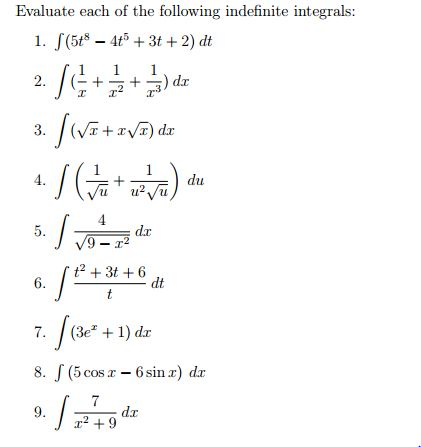
\includegraphics[width=0.9\linewidth]{Question19integration1}
\end{figure}
%============================================================= %
\newpage
\section*{MA4702 Integration}

\subsection*{Question 33 : Integration}
% - http://en.wikibooks.org/wiki/Calculus/Integration/Exercises
Using appropriate substitutions, evaluate the indefinite integrals:
\begin{multicols}{2}
	\begin{itemize}
		
		\item[(i)] \[\int (x^2-2)^{2}\, dx\]
		\item[(ii)] \[\int 8x^3\, dx\]
		\item[(iii)]\[ \int (4x^2+11x^3)\, dx\]
		\item[(iv)] \[\int (31x^{32}+4x^3-9x^4) \,dx\]
		\item[(v)] \[\int 5x^{-2}\, dx\]
	\end{itemize}
\end{multicols}
%=========================== %
Using appropriate substitutions, evaluate the indefinite integrals:
\begin{multicols}{2}
	\begin{itemize}
	
	\item[(i)]	
	\[\int 3x^2 (x^3+1)^5 \, dx\]
	
	\item[(ii)]
	\[\int x^4 \sin(x^5) \, dx\]
	\end{itemize}
\end{multicols}
\bigskip

\begin{figure}[h!]
	\centering
	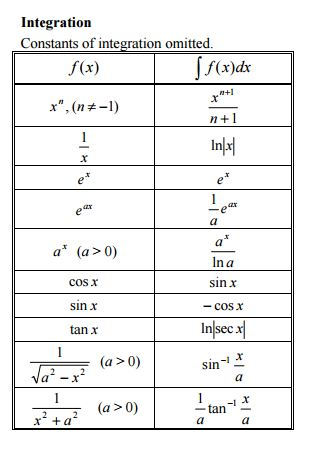
\includegraphics[width=0.55\linewidth]{integrationtabless}
\end{figure}



%Example
%
%\[\int_1^3 9 dx = 9(3-1)=9\cdot 2 = 18.\]
%\[\int_{-2}^6 11 dx = 11(6-(-2))=11\cdot 8 = 88.\]
%\[\int_{2}^{17} 0 dx = 0\cdot(17-2) =0.\]


Addition and Subtraction Rules of Integration
\[\int_a^b (f(x) + g(x)) dx = \int_a^b f(x) dx + \int_a^b g(x) dx.\]

\[\int_a^b (f(x) - g(x)) dx = \int_a^b f(x) dx - \int_a^b g(x) dx.\]


%Example
%
%From above $\int_1^3 9 dx =  18$ and $\int_1^3 2x^2 dx = \frac{52}{3} $so
%
%\[\int_1^3 (2x^2 + 9)dx = \int_1^3 2x^2 dx + \int_1^3 9 dx = \frac{52}{3} + 18 = \frac{106}{3},\]
%\[\int_1^3 (2x^2 - 9)dx = \int_1^3 2x^2 dx - \int_1^3 9 dx = \frac{52}{3} - 18 = -\frac{2}{3}.\]
%
%Example
%
%\[\int_0^2 4x^2 + 14 dx = 4\int_0^2 x^2 dx + \int_0^2 14 dx = 4 \cdot \frac{1}{3}(2^3-0^3) + 2 \cdot 14 = \frac{32}{3} + 28 = \frac{116}{3}.\]


%============================================================== %

\subsection*{The Power Rule for Integration}
The power rule for derivatives can be reversed to give us a way to handle integrals of powers of x. Since

\[\frac{d}{dx} x^n = n x^{n-1},\]

we can conclude that

\[\int n x^{n-1} \, dx = x^n + C,\]

or, a little more usefully,

\[\int x^n \, dx = \frac{x^{n+1}}{n+1} + C\]
\subsection*{Question 34 : Integration}
% - http://en.wikibooks.org/wiki/Calculus/Integration/Exercises
Evaluate the following:
\begin{multicols}{2}
	\begin{itemize}
		
		\item[(i)] \[\int (x^2-2)^{2}\, dx\]
		\item[(ii)] \[\int 8x^3\, dx\]
		\item[(iii)]\[ \int (4x^2+11x^3)\, dx\]
		\item[(iv)] \[\int (31x^{32}+4x^3-9x^4) \,dx\]
		\item[(v)] \[\int 5x^{-2}\, dx\]
	\end{itemize}
\end{multicols}







%===============================================================================%

\subsection*{Question 35 : Introduction to Integration}
\subsubsection*{Part A}
Using appropriate substitutions, evaluate the indefinite integrals:

\begin{multicols}{2}
	\begin{enumerate}[(i)]
		
		\item 
		\[ \int (s - 4)^5 ds \]
		\item 
		\[ \int 
		\frac{3}{(x + 1)^4 }dx\]
		\item 
		\[\int 
		(2y + 3)(y^2 + 3y + 2)^2 dy\]
		
	\end{enumerate}
\end{multicols}
%========================================================================== %
\subsubsection*{Part B}
Evaluate the following indefinite integrals using partial fractions:
\begin{multicols}{2}
	\begin{enumerate}[(i)]
		
		\item \[ \int \frac{x}{x^2-9} dx  \]
		
		\item \[ \int \frac{x}{x^2 - 4x + 3} dx  \]
		
		\item \[ \int \frac{x}{x^2 - 4x + 3} dx  \]
		
	\end{enumerate}
\end{multicols}


%============================================================================================= %





%============================================================================= %
% - http://wiki.ubc.ca/Partial_Derivatives
\newpage
\subsection*{Question 36 : Definite Integrals}
Evaluate the following definite integrals 


\begin{multicols}{2}
	\begin{enumerate}[(i)]
		\item \[ \int^{2}_{1} (x^2-1) dx \]
		
		%	\item  \[ \int^{2}_{0} x^2+1 dx \]
		
		\item \[ \int^{\frac{\pi}{2}}_{0} \cos x dx \]
		
		\item \[ \int^{\pi}_{0} \cos x dx \]
		
		\item \[ \int^{2}_{1} (y^2 - y^{-2}) dy \]
		
		% - \item \[ \int^{2}_{1} y^2+y{-2} dx \]
		
		\item \[ \int^{1}_{-3} (6x^2 -5x + 2)dx \]
		
		% - \item \[ \int^{1}_{-3} \int 6x^2 -5x +2 dx \]
		
		
		
		\item \[ \int^0_4 \sqrt{t}(t-2) dt \]
		
		% - \item \[ \int^{0}_{4} \sqrt{t}(t-2) dt \]
		
		
		% - http://tutorial.math.lamar.edu/Classes/CalcI/ComputingDefiniteIntegrals.aspx#Int_CompDef_Ex3a
		
		% -	\item \[ \int^{2}_{1} \frac{2w^5 - w + 3}{w^2} dw \]
		
		% - \item \[ \int^{2}_{1} dR \]
	\end{enumerate}
\end{multicols}
%-------------------------------------------------%

\begin{framed}
	\textbf{Hint:} 
	\[ \int \sqrt{t}(t-2) dt \]
	
	\[ \sqrt{t}(t-2) = t^{1/2} \times (t - 2) = t^{3/2} - 2t^{1/2}\]
	
\end{framed}
%--------------------------------------------------%


% \[ x^2 - 4x + 3 = (x-1)(x-3) \]

% \[ \int \frac{}{} dx \]

%============================================================================================= %
\subsection*{Question 37 : Definite Integrals}
\begin{figure}[h!]
	\centering
	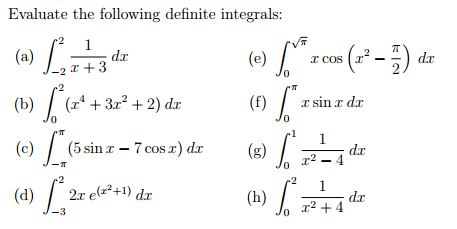
\includegraphics[width=0.8\linewidth]{Question25}
\end{figure}
\newpage
%============================================================================================= %
%=============================================================================================================== %
% Appilcations of Integration
\subsection*{Question 38 : Integration by Parts}
Evaluate the following using integration by parts.

\begin{multicols}{2}
	\begin{enumerate}[(i)]
		\item \[ \int -4\ln\left(x\right)dx\]
		% -4x\ln\left(x\right)+4x+C
		
		\item \[ \int\left(-7x+38\right)\cos\left(x\right)dx\]
		% \left(-7x+38\right)\sin\left(x\right)-7\cos\left(x\right)+C
		
		\item  \[\int_0^\frac{\pi}{2}\left(-6x+45\right)\cos\left(x\right)dx\]
		
		% -3\pi+51
		
		\item \[ \int\left(5x+1\right)\left(x-6\right)^4 dx\]
		
		% \frac{\left(5x+1\right)\left(x-6\right)^5}{5}-\frac{\left(x-6\right)^6}{6}+C
		
		\item \[ \int_{-1}^1 \left(2x+8\right)^3\left(-x+2\right)dx\]
		
		% \frac{9584}{5}
		
		\item \[ \int \sin\left(x\right) e^x\, dx \] 
		% \frac 1 2 e^x\left(\sin\left(x\right) - \cos\left(x\right) \right) +C
	\end{enumerate}
\end{multicols}




%==============================================================================%




\subsection*{Question 39 : Integration by Parts}
Revision Week Exercises
\begin{figure}[h!]
	\centering
	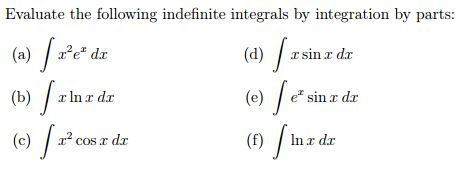
\includegraphics[width=0.7\linewidth]{Question26integrationbyparts}
\end{figure}
%========================================================================== %

\subsection*{Question 40 : Integration by Parts}
\begin{framed}
	\textbf{Formula:} \\ If u and v are functions of x that have continuous derivatives,
	then
	\[\int udv = uv - \int vdu\]
\end{framed}
\subsubsection*{The LIPET rule}
It is considered a rule of thumb to remember the acronym \textbf{LIPET}
when performing integration by parts. This acronym will help you to determine
what to use as $u$. 


\begin{description}
	\item[L]-logarithms, 
	\item[I]-inverse trigonometric functions,
	\item[P]-polynomials (i.e. $x$, $x^2$) , 
	\item[E]-exponentials (i.e. $e^x$, $e^{3x}$), 
	\item[T]-trigonometric functions.
\end{description}

%=================================%
\begin{framed}
	\begin{itemize}
		\item
		$\cosh(x)$ is both the derivative and integral of $\sinh(x)$
		
		\item
		$\sinh(x)$ is both the derivative and integral of $\cosh(x)$
	\end{itemize}
\end{framed}
\bigskip
\subsection*{Question 41 : Definite Integrals}
\begin{framed}
	{\large
		\noindent \textbf{Exercise}: Evaluate the following definite integral
		\[ \int^{3}_{1} \frac{x}{3}  dx \]
		\textbf{Solution}
		\[ \int^{3}_{1} \frac{x}{3}  dx  = \left[\frac{x^4}{4}\right]^{3}_{1}= \frac{81}{4} - \frac{1}{4} = 20\]
	}
\end{framed}
\newpage
%=========================== %
\begin{framed}
	{\large
		\noindent \textbf{Exercise}: Evaluate the following definite integral
		
		\[ \int^3_1 \frac{x^2 - 4x + 3}{x-3}  dx \] 
		
		\noindent	Factorize the numerator $x^2 - 4x + 3 = (x-1)(x-3)$
		
		
		Treat it as an indefinite integral for time being.			
		\[ \int \frac{x^2 - 4x + 3}{x-3}  dx = \int \frac{(x-1)(x-3)}{x-3}  dx  = \int (x-1) dx = \frac{x^2}{2} -x +c\] 
		
		\[ \left[ \frac{x^2}{2} -x\right]^{3}_{1} = (4.5-3)-(0.5-1) = 2\]
	}
\end{framed}


\subsection*{Question 42 : Integration by Parts (Exam Standard)}	
the following questions are from previous past papers. Please be advised of the notes below.
\begin{enumerate}[(i)]
	\item (2005) Use integration by parts to find $\displaystyle{\int xe^xdx}$ 
	
	\item (2006) Use integration by parts to find $\displaystyle{\int x ln(x) dx}$ 
	
	\item (2007) Use integration by parts to find $\displaystyle{\int x sinh(x) dx}$ 
	
	\item (2008) Use integration by parts to find $\displaystyle{\int x cos(x) dx}$ 
	
	\item (2009) Use integration by parts to find $\displaystyle{\int x cosh(x) dx}$ 
	
	\item (2010) Use integration by parts to find $\displaystyle{\int xe^xdx}$ 
\end{enumerate}

% - http://www.math.uri.edu/~adamgilbert/Documents/Calculus/Notes/MTH142/IntegrationByParts.pdf
\newpage
\begin{framed}
	\noindent \textbf{Important:	}
	\begin{itemize}
		\item You should expect to see hyperbolic functions (i.e. $\cosh(x)$ and $\sinh(x)$)  in the end of semester exam. 
		\item However you should expect to see terms like $ x^2$, $e^{2x}$ and $ \ln(x)$, as well as what was in previous exams.
		\item \textbf{VERY Important:} Make sure you know how to integrate and differentiate expressions of the form $e^{ax}$, $\cos(ax)$, $\cosh(ax)$ , $\sin(ax)$ and $\sinh(ax)$. 
	\end{itemize}
\end{framed}

%================================================= %
\subsection*{Question 43 : Definite Integrals}
Evaluate the following definite integrals 

\begin{enumerate}[(i)]
	
	\item 
	% - Lecture Notes Definite Integral
	% Examples 5 to 7
	Find the area between $f(x) = x^2 + 4x $ and the $x-$axis between 
	$x=-4$   and $ x=3$.
	
	\item Calculate the following:
	\[ \int^{1}_{0} \frac{4x^3}{x^4+1} dx \]
	
	
	\item Evaluate 
	
	\[ \int^{\frac{\pi}{2}}_{0} \cos^4(x) \sin(x) dx \]
\end{enumerate}

%=================================================================================== %



%===============================================%
\subsection*{Question 34 : Simpson's Rule}
\begin{itemize}
	\item[(i)] 
	Use Simpson’s rule with 4 equal subintervals to find an approximation       
	for  \[ \int^{2}_{0} \sqrt{1+3x^2} dx \]  .	
	\item[(ii)] Use Simpson’s rule with 4 equal subintervals to find an approximation       
	for    \[ \int^2_0 \sqrt{1+x^2} dx \] 
\end{itemize}
%============================================================================================= %

		\subsection*{Question 28 : Integration and Numerical Integration}
		
		\begin{enumerate}
			\item \textbf{Integrations by Parts} \\ Evaluate the following expression, using the Integration by Parts" technique
			
			%% - http://tutorial.math.lamar.edu/Classes/CalcII/IntegrationByParts.aspx
			
			\begin{itemize}
				\item[(i)] \[ \int x \sqrt{x+1} dx \]
				\item[(ii)] \[ \int x^5 \sqrt{x^3+1} dx \]
				\item[(ii)] \[ \int e^x cos(x) dx \]
			\end{itemize}
			%=================================================================================== %
			\item \textbf{Trapezoidal Rule}
			% % - http://www.intmath.com/integration/5-trapezoidal-rule.php
			\item \textbf{Simpson's Rule}
		\end{enumerate}
		
		
		
		%======================================================================================================= %
		\begin{center}
			\textbf{Tutorial Sheet 5}
		\end{center}
		\newpage
		Which of the following functions are well defined functions? If the function is not well defined, give a counterexample showing that it is not.
		\begin{multicols}{2}
			\begin{enumerate}
				\item $f: \mathbb{R} \to \mathbb{R},\quad f(x)=x^2+1$
				\item $f: \mathbb{R}^+ \to \mathbb{R}^+,\quad f(x)=x^2+1$
				\item $f: \mathbb{R}^+ \to [1,10],\quad f(x)=x^2+1$
				\item $f: \mathbb{R}^+ \to [1,\infty),\quad f(x)=x^2+1$
				\item $f: \mathbb{R}^+ \to \mathbb{R}^+,\quad f(x)=\sqrt[+]{x}$
				\item $f: \mathbb{R}^- \to \mathbb{R}^-,\quad f(x)=\sqrt[+]{x}$
				\item $f: \mathbb{R}^+ \to \mathbb{R}^-,\quad f(x)=\sqrt[+]{x}$
				\item $f: \mathbb{R}^+ \to \mathbb{R},\quad f(x)=\sqrt[+]{x}$
				\item $f: \mathbb{R} \to \mathbb{R},\quad f(x)=\frac{1}{x}$
				\item $f: \mathbb{R}\setminus\{0\} \to \mathbb{R},\quad f(x)=\frac{1}{x}$
				\item $f: \mathbb{R}^+\setminus\{0\} \to \mathbb{R},\quad f(x)=\frac{1}{x}$
				\item $f: \mathbb{R}^+\setminus\{0\} \to \mathbb{R},\quad f(x)=\frac{1}{x-1}$
				\item $f: \mathbb{R}^+\setminus\{1\} \to \mathbb{R}^+,\quad f(x)=\frac{1}{x-1}$
				\item $f: \mathbb{R} \to \mathbb{R},\quad f(x)=e^x$
				\item $f: \mathbb{R} \to \mathbb{R}^+,\quad f(x)=e^x-1$
				\item $f: \mathbb{R} \to \mathbb{R},\quad f(x)=\ln(x)$
				\item $f: \mathbb{R}^+\setminus \{0\} \to \mathbb{R}^+,\quad f(x)=\ln(x)$
				\item $f: \mathbb{R}^+\setminus \{0\} \to \mathbb{R},\quad f(x)=\ln(x)$
				\item $f: (1,\infty) \to \mathbb{R},\quad f(x)=\ln(x+1)$
			\end{enumerate}
		\end{multicols}
		
		\newpage
		For each of the following well defined functions, say whether the function is one-to-one, onto, or invertible. In the case of invertible functions, give the inverse function. In the case of non-invertible functions, modify the domain and codomain of the functions to make them invertible and give the corressponding inverse function.
		\begin{multicols}{2}
			\begin{enumerate}
				\item $f: \mathbb{R} \to \mathbb{R},\quad f(x)=2x+4$
				\item $f: \mathbb{R} \to \mathbb{R},\quad f(x)=x$
				\item $f: \mathbb{R} \to \mathbb{R},\quad f(x)=x^2$
				\item $f: \mathbb{R} \to \mathbb{R}^+,\quad f(x)=x^2+4$
				\item $f: \mathbb{R}^+ \to \mathbb{R},\quad f(x)=\sqrt[+]{x}$
				\item $f: \mathbb{R}\setminus\{0\} \to \mathbb{R},\quad f(x)=\frac{1}{x}$
				\item $f: \mathbb{R} \to \mathbb{R},\quad f(x)=e^x$
				\item $f: \mathbb{R}^+ \to [1,\infty),\quad f(x)=e^x$
				\item $f: \mathbb{R}^+ \to \mathbb{R}^+,\quad f(x)=e^x+1$
				\item $f: \mathbb{R} \to \mathbb{R},\quad f(x)=\sin(x)$
				\item $f: (\text{-}\pi,\pi) \to [\text{-}1,1],\  f(x)=\sin(x)$
				\item $f: (\text{-}\frac{\pi}{2},\frac{\pi}{2}) \to [\text{-}1,1],\  f(x)=\sin(x)$
			\end{enumerate}
		\end{multicols}
		%	\subsection*{Sketching Question}
		%	Graph the well defined function $f: \mathbb{R} \to \mathbb{R}, \ f(x)=\cosh(x)$ on the interval $[-2,2]$. Based on the graph, give a suitable domain and codomain of the function to make it invertible.
		%	
		%================================================================ %	


\bigskip

	\subsection*{Question 9 : Change of Base Formula}
	% % - http://www.mathwords.com/c/change_of_base_formula.htm
	A formula that allows you to rewrite a logarithm in terms of logs written with another base. This is especially helpful when using a calculator to evaluate a log to any base other than 10 or e.
	
	
	
	Assume that x, a, and b are all positive. Also assume that $a \neq 1$, $b \neq 1$.
	
	Change of base formula: 
	
	\[  \log_a x =  \frac{\log_{b} x }{ \log_{b} a } \]
	
	\noindent \textbf{Example 1: }
	
	\[  =  \frac{\log_{32} }{ \log_{16} }  =  \frac{\log_{32} }{ \log_{16} } \]
	
	\noindent \textbf{Example 2:  }  \\ (note that $2^{4} = 16$ and $2^{5} = 32$ )
	
	\[  \log_2 3 =  \frac{\log_{32} }{ \log_{16} } \]
	
	
	\noindent \textbf{Example 3: }
	\[  \log_a x =  \frac{\log_{32} }{ \log_{16} } \]
	
	
	
	\bigskip
	
	
	%==============================================================================%
	\begin{itemize}
		\item	Trigonometric Functions
		\item   Unit Circle
		
	\end{itemize}

\subsection*{Question 29 : Maclaurin Series}
\begin{itemize}
	\item A MacLaurin series of a function f(x) for which a derivative may be taken of the function or any of its derivatives at 0 is the power series
	
	
	\[f(0) + f^{\prime}(0) + \frac{f^{\prime \prime}(0)}{2!} + \frac{f^{\prime \prime}(0)}{2!} \]
	which can be written in the more compact sigma, or summation, notation as
	\begin{figure}[h!]
		\centering
		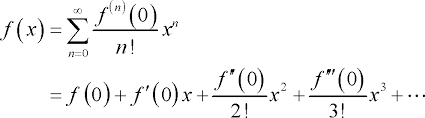
\includegraphics[width=0.25\linewidth]{MaclaurinFormula.png}
	\end{figure}
	
	where $n!$ denotes the factorial of n and $f^{(n)}(0)$ denotes the nth derivative of f evaluated at the point 0. 
	\item The derivative of order zero f is defined to be f itself and $(x)^0$ and 0! are both defined to be 1.
	\item \textit{(Relation to Taylor Series: Maclaurin series is a Taylor series expansion of a function about 0. )}
	
\end{itemize}


\begin{itemize}
	\item[(i)] Derive the Maclaurin Expansion of $sin(t)$.
\end{itemize}
\begin{figure}[h!]
	\centering
	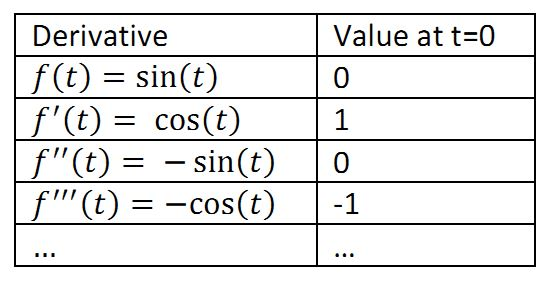
\includegraphics[width=0.45\linewidth]{macl1}
\end{figure}
\begin{figure}[h!]
	\centering
	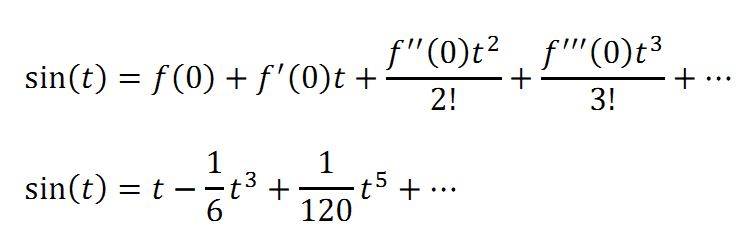
\includegraphics[width=0.65\linewidth]{macl2}
\end{figure}


%
%\begin{itemize}
%	\item[(i)] Derive the Maclaurin Expansion of $cos(t)$.
%\end{itemize}
%==========================================================================%

\begin{itemize}
	\item[(i)]Find the Maclaurin series of $f(x) = cos(x)$ up to and including the term
	containing $x^4$.
	\\
	Use your answer to estimate the value of $cos(1)$
	\item[(ii)] Find the Maclaurin series of $f(x) =e^x$ up to and including the term containing
	$x^6$
	\item[(iii)] Use your answer from part (ii) to estimate the value of $e^3$, $e^{0.5}$ and $e^{-1}$
\end{itemize}
\newpage

\subsection*{Question 50}

%Solve for $\partial g/\partial x (3,2)$ and $\partial g/\partial y (3,2)$ if $g(x,y) = xye^$.

\subsubsection*{Solution :}
\[\partial g/\partial x = (xy)\times(2xe^{x^2}) + ye^{x^2}\]
\[= 2ye^{x^2} + ye^{x^2} =ye^{(2+1)}\]


\[\partial g/\partial x (3,2) = 2e^(2+1)\]
= 2(19)
= 38

%\[\partial g/\partial y = xe^\]
\[\partial g/\partial y (3,2) = 3\]

%============================================================================%
Example 4 :

Find the rectangular box of least surface area that has volume 1000.
Solution :
\begin{itemize}
	\item Volume = 1000 = xyz
	\item Surface Area = 2xz + 2yz + 2xy
	\item z = 1000/xy
	\item S = 2x(1000/xy) + 2y(1000/xy) + 2xy
	\item = 2000/y + 2000/x + 2xy *need to minimize this*
\end{itemize}
%---------------------------------%
Solve for $\partial S/\partial x = 0 and \partial S/\partial y = 0$
\begin{itemize}
	\item $\partial S/\partial x = -2000/ + 2y = 0$
	\item $\partial S/\partial y = -2000/ + 2x = 0$
	\item $y = 1000/ and x = 1000/$
	\item $y() = 0$
\end{itemize}

Therefore, y = 0 or -1000 = 0
So, y = 10 and x = 10.
Using the second derivative test, S does have a local minimum at (10, 10).








%============================================================== %

\section*{Appendices}
\subsection*{Limits}	
% %- https://en.wikibooks.org/wiki/Calculus/Limits/An_Introduction_to_Limits
\begin{itemize}
	\item \textbf{Example 1}\\
	Find the limit $\lim_{x\to 2} {4x^3}$.
	
	We need to simplify the problem, since we have no rules about this expression by itself. We know from the identity rule above that $\lim_{x\to 2} {x} = 2$.\\ \bigskip By the power rule, \[\lim_{x\to 2} {x^3} = \left(\lim_{x\to 2} x\right)^3 = 2^3 = 8\]. Lastly, by the scalar multiplication rule, we get \[\lim_{x\to 2} {4x^3} = 4\lim_{x\to 2} x^3=4 \cdot 8=32\].
	
	\item \textbf{Example 2} \\
	Find the limit $\lim_{x\to 2} [4x^3 + 5x +7].$
	
	To do this informally, we split up the expression, once again, into its components. As above,$\lim_{x\to 2} 4x^3=32$.
	
	Also $\lim_{x\to 2} 5x = 5\cdot\lim_{x\to 2} x = 5\cdot2=10 and \lim_{x\to 2} 7 =7$. \\ Adding these together gives
	
	\[\lim_{x\to 2} 4x^3 + 5x +7 = \lim_{x\to 2} 4x^3 + \lim_{x\to 2} 5x + \lim_{x\to 2} 7 = 32 + 10 +7 =49.\]
	
	\item \textbf{Example 3} \\
	Find the limit $\lim_{x\to 2}\frac{4x^3 + 5x +7}{(x-4)(x+10)}$.
	
	From the previous example the limit of the numerator is \[\lim_{x\to 2} 4x^3 + 5x +7 =49.\] The limit of the denominator is
	
	\[\lim_{x\to 2} (x-4)(x+10) = \lim_{x\to 2} (x-4) \cdot \lim_{x\to 2} (x+10) = (2-4)\cdot(2+10)=-24.\]
	As the limit of the denominator is not equal to zero we can divide. This gives
	
	\[\lim_{x\to 2}\frac{4x^3 + 5x +7}{(x-4)(x+10)} = -\frac{49}{24}.\]
	\item Example 4 \\
	Find the limit $\lim_{x\to 4}\frac{x^4 - 16x + 7}{4x-5}.$
	
	We apply the same process here as we did in the previous set of examples;
	
	\[\lim_{x\to 4}\frac{x^4 - 16x + 7}{4x-5} = \frac{\lim_{x\to 4} (x^4 - 16x + 7)} {\lim_{x\to 4} (4x-5)} = \frac{\lim_{x\to 4} (x^4) - \lim_{x\to 4} (16x) + \lim_{x\to 4} (7)} {\lim_{x\to 4} (4x) - \lim_{x\to 4} 5}.\]
	We can evaluate each of these; 
	\[\lim_{x\to 4} (x^4) = 256,\]
	
	\[\lim_{x\to 4} (16x) = 64,\]
	
	\[\lim_{x\to 4} (7) = 7,\]
	
	\[\lim_{x\to 4} (4x) = 16\]
	and  $\lim_{x\to 4} (5) = 5$. Thus, the answer is $\frac{199}{11}$.
	
	\item \textbf{Example 5} \\
	Find the limit $\lim_{x\to 2}\frac{x^2 - 3x + 2}{x-2}.$
	
	In this example, evaluating the result directly will result in a division by zero. While you can determine the answer experimentally, a mathematical solution is possible as well.
	
	First, the numerator is a polynomial that may be factored: \[\lim_{x\to 2}\frac{(x-2)(x-1)}{x-2}\]
	
	Now, you can divide both the numerator and denominator by (x-2): \[\lim_{x\to 2} (x-1) = (2-1) = 1\]
	
	
	
	\item \textbf{Example 6} \\
	Find the limit $\lim_{x\to 0}\frac{1-\cos x}{x}$.
	
	To evaluate this seemingly complex limit, we will need to recall some sine and cosine identities. We will also have to use two new facts. First, if f(x) is a trigonometric function (that is, one of sine, cosine, tangent, cotangent, secant or cosecant) and is defined at a, then  $\lim_{x\to a} f(x) = f(a)$.
	
	Second, $\lim_{x\to 0}\frac{\sin x}{x} = 1$. This may be determined experimentally, or by applying L'Hôpital's rule, described later in the book.
	
	To evaluate the limit, recognize that  $1 - \cos x$ can be multiplied by  $1+\cos x$ to obtain  $(1-\cos^2 x)$ which, by our trig identities, is  $\sin^2 x$. So, multiply the top and bottom by  $1+\cos x$. (This is allowed because it is identical to multiplying by one.) This is a standard trick for evaluating limits of fractions; multiply the numerator and the denominator by a carefully chosen expression which will make the expression simplify somehow. In this case, we should end up with:
	
	\begin{align}\lim_{x\to 0} \frac{1-\cos x}{x} &=& \lim_{x\to 0} \left(\frac{1-\cos x}{x} \cdot \frac{1}{1}\right) \\
	&=& \lim_{x\to 0} \left(\frac{1-\cos x}{x} \cdot \frac{1 + \cos x} {1+ \cos x}\right) \\
	&=& \lim_{x\to 0}\frac{(1 - \cos x) \cdot 1 + (1 - \cos x) \cdot \cos x} {x \cdot (1+ \cos x)} \\
	&=& \lim_{x\to 0}\frac{1 - \cos x + \cos x - \cos^2 x}{x \cdot (1+ \cos x)} \\
	&=& \lim_{x\to 0}\frac{1 - \cos^2 x} {x \cdot (1+ \cos x)} \\
	&=& \lim_{x\to 0}\frac{\sin^2 x} {x \cdot (1+ \cos x)} \\
	&=& \lim_{x\to 0} \left(\frac{\sin x} {x} \cdot \frac{\sin x} {1+ \cos x}\right)\end{align} \nonumber.
	
	Our next step should be to break this up into $\lim_{x\to 0}\frac{\sin x}{x} \cdot \lim_{x\to 0} \frac{\sin x}{1+\cos x}$ by the product rule. As mentioned above, $\lim_{x\to 0} \frac{\sin x} {x} = 1.$
	
	Next, $ \lim_{x\to 0} \frac{\sin x} {1+\cos x} = \frac{\lim_{x\to 0}\sin x} {\lim_{x\to 0} (1+\cos x)} = \frac{0} {1 + \cos 0} = 0$.
	
	Thus, by multiplying these two results, we obtain 0.
	
\end{itemize}	


%=======================================================================


\end{document}